%%%%%%%%%%%%%%%%%%%%%%%%%%%%%%%%%%%%%%%%%
% Wenneker Article
% LaTeX Template
% Version 2.0 (28/2/17)
%
% This template was downloaded from:
% http://www.LaTeXTemplates.com
%
% Authors:
% Vel (vel@LaTeXTemplates.com)
% Frits Wenneker
%
% License:
% CC BY-NC-SA 3.0 (http://creativecommons.org/licenses/by-nc-sa/3.0/)
%
%%%%%%%%%%%%%%%%%%%%%%%%%%%%%%%%%%%%%%%%%

%----------------------------------------------------------------------------------------
%	PACKAGES AND OTHER DOCUMENT CONFIGURATIONS
%----------------------------------------------------------------------------------------
%f
\documentclass[10pt, a4paper]{article} % 10pt font size (11 and 12 also possible), A4 paper (letterpaper for US letter) and two column layout (remove for one column)

%%%%%%%%%%%%%%%%%%%%%%%%%%%%%%%%%%%%%%%%%
% Wenneker Article
% Structure Specification File
% Version 1.0 (28/2/17)
%
% This file originates from:
% http://www.LaTeXTemplates.com
%
% Authors:
% Frits Wenneker
% Vel (vel@LaTeXTemplates.com)
%
% License:
% CC BY-NC-SA 3.0 (http://creativecommons.org/licenses/by-nc-sa/3.0/)
%
%%%%%%%%%%%%%%%%%%%%%%%%%%%%%%%%%%%%%%%%%

%----------------------------------------------------------------------------------------
%	PACKAGES AND OTHER DOCUMENT CONFIGURATIONS
%----------------------------------------------------------------------------------------

\usepackage[english]{babel} % English language hyphenation

\usepackage{microtype} % Better typography

\usepackage{amsmath,amsfonts,amsthm} % Math packages for equations

\usepackage[svgnames]{xcolor} % Enabling colors by their 'svgnames'

\usepackage[hang, small, labelfont=bf, up, textfont=it]{caption} % Custom captions under/above tables and figures

\usepackage{booktabs} % Horizontal rules in tables

\usepackage{lastpage} % Used to determine the number of pages in the document (for "Page X of Total")

\usepackage{graphicx} % Required for adding images

\usepackage{enumitem} % Required for customising lists
\setlist{noitemsep} % Remove spacing between bullet/numbered list elements

\usepackage{sectsty} % Enables custom section titles
\allsectionsfont{\usefont{OT1}{phv}{b}{n}} % Change the font of all section commands (Helvetica)

%----------------------------------------------------------------------------------------
%	MARGINS AND SPACING
%----------------------------------------------------------------------------------------

\usepackage{geometry} % Required for adjusting page dimensions

\geometry{
	top=1cm, % Top margin
	bottom=1.5cm, % Bottom margin
	left=2cm, % Left margin
	right=2cm, % Right margin
	includehead, % Include space for a header
	includefoot, % Include space for a footer
	%showframe, % Uncomment to show how the type block is set on the page
}

\setlength{\columnsep}{7mm} % Column separation width

%----------------------------------------------------------------------------------------
%	FONTS
%----------------------------------------------------------------------------------------

\usepackage[T1]{fontenc} % Output font encoding for international characters
\usepackage[utf8]{inputenc} % Required for inputting international characters

\usepackage{XCharter} % Use the XCharter font

%----------------------------------------------------------------------------------------
%	HEADERS AND FOOTERS
%----------------------------------------------------------------------------------------

\usepackage{fancyhdr} % Needed to define custom headers/footers
\pagestyle{fancy} % Enables the custom headers/footers

\renewcommand{\headrulewidth}{0.0pt} % No header rule
\renewcommand{\footrulewidth}{0.4pt} % Thin footer rule

\renewcommand{\sectionmark}[1]{\markboth{#1}{}} % Removes the section number from the header when \leftmark is used

%\nouppercase\leftmark % Add this to one of the lines below if you want a section title in the header/footer

% Headers
\lhead{} % Left header
\chead{\textit{\thetitle}} % Center header - currently printing the article title
\rhead{} % Right header

% Footers
\lfoot{} % Left footer
\cfoot{} % Center footer
\rfoot{\footnotesize Page \thepage\ of \pageref{LastPage}} % Right footer, "Page 1 of 2"

\fancypagestyle{firstpage}{ % Page style for the first page with the title
	\fancyhf{}
	\renewcommand{\footrulewidth}{0pt} % Suppress footer rule
}

%----------------------------------------------------------------------------------------
%	TITLE SECTION
%----------------------------------------------------------------------------------------

\newcommand{\authorstyle}[1]{{\large\usefont{OT1}{phv}{b}{n}\color{DarkRed}#1}} % Authors style (Helvetica)

\newcommand{\institution}[1]{{\footnotesize\usefont{OT1}{phv}{m}{sl}\color{Black}#1}} % Institutions style (Helvetica)

\usepackage{titling} % Allows custom title configuration

\newcommand{\HorRule}{\color{DarkGoldenrod}\rule{\linewidth}{1pt}} % Defines the gold horizontal rule around the title

\pretitle{
	\vspace{-30pt} % Move the entire title section up
	\HorRule\vspace{10pt} % Horizontal rule before the title
	\fontsize{32}{36}\usefont{OT1}{phv}{b}{n}\selectfont % Helvetica
	\color{DarkRed} % Text colour for the title and author(s)
}

\posttitle{\par\vskip 15pt} % Whitespace under the title

\preauthor{} % Anything that will appear before \author is printed

\postauthor{ % Anything that will appear after \author is printed
	\vspace{10pt} % Space before the rule
	\par\HorRule % Horizontal rule after the title
	\vspace{20pt} % Space after the title section
}

%----------------------------------------------------------------------------------------
%	ABSTRACT
%----------------------------------------------------------------------------------------

\usepackage{lettrine} % Package to accentuate the first letter of the text (lettrine)
\usepackage{fix-cm}	% Fixes the height of the lettrine

\newcommand{\initial}[1]{ % Defines the command and style for the lettrine
	\lettrine[lines=3,findent=4pt,nindent=0pt]{% Lettrine takes up 3 lines, the text to the right of it is indented 4pt and further indenting of lines 2+ is stopped
		\color{DarkGoldenrod}% Lettrine colour
		{#1}% The letter
	}{}%
}

\usepackage{xstring} % Required for string manipulation

\newcommand{\lettrineabstract}[1]{
	\StrLeft{#1}{1}[\firstletter] % Capture the first letter of the abstract for the lettrine
	\initial{\firstletter}\textbf{\StrGobbleLeft{#1}{1}} % Print the abstract with the first letter as a lettrine and the rest in bold
}

%----------------------------------------------------------------------------------------
%	BIBLIOGRAPHY
%----------------------------------------------------------------------------------------

\usepackage[backend=bibtex,style=authoryear,natbib=true]{biblatex} % Use the bibtex backend with the authoryear citation style (which resembles APA)

\addbibresource{Bibliography.bib} % The filename of the bibliography

\usepackage[autostyle=true]{csquotes} % Required to generate language-dependent quotes in the bibliography
 % Specifies the document structure and loads requires packages

%----------------------------------------------------------------------------------------
%	ARTICLE INFORMATION
%----------------------------------------------------------------------------------------

\title{Impact of interpersonal relation of dominance in collaborative negotiation} % The article title
%
%\author{
%	\authorstyle{John Marston\textsuperscript{1,2,3} and Bonnie MacFarlane\textsuperscript{2,3}} % Authors
%	\newline\newline % Space before institutions
%	\textsuperscript{1}\institution{Universidad Nacional Autónoma de México, Mexico City, Mexico}\\ % Institution 1
%	\textsuperscript{2}\institution{University of Texas at Austin, Texas, United States of America}\\ % Institution 2
%	\textsuperscript{3}\institution{\texttt{LaTeXTemplates.com}} % Institution 3
%}

% Example of a one line author/institution relationship
%\author{\newauthor{John Marston} \newinstitution{Universidad Nacional Autónoma de México, Mexico City, Mexico}}

\date{\today} % Add a date here if you would like one to appear underneath the title block, use \today for the current date, leave empty for no date

%----------------------------------------------------------------------------------------

\begin{document}

\maketitle % Print the title

\thispagestyle{firstpage} % Apply the page style for the first page (no headers and footers)

%----------------------------------------------------------------------------------------
%	ABSTRACT
%----------------------------------------------------------------------------------------

\lettrineabstract{}

%----------------------------------------------------------------------------------------
%	ARTICLE CONTENTS
%----------------------------------------------------------------------------------------

\section{Introduction}

%------------------------------------------------
Affective computing is an emerging field of research that ranges from computer science to psychology, and from social sciences to cognitive sciences. This field of research focuses on building intelligent conversational agents interacting with human users. These agents are capable of perceiving, recognizing and stimulating social affects involved in human interactions.

Social and emotional behaviors play a crucial role in our daily lives. They affect our decision-making process, our verbal and nonverbal behaviors during interactions. Therefore, extending conversational agents with this social-emotional intelligence will improve the quality of interactions. As a results, it increases the acceptability and credibility of conversational agents. 

Therefore, we witness an increasing emergence of social conversational agents in various application areas.  These agents play different roles ranging from artificial companion \cite{ring2013addressing,sidner2013always}, virtual patient \cite{kenny2007virtual,kleinheksel2017virtual} or tutor for \emph{e-learning}  \cite{kerly2008calmsystem,kerry2009conversational}.

Interactions between a conversational agent and a human user generally take place in a collaborative environment where the agent and user share common objectives and interests. 
Consequently, they are led to collaborate, through their interaction, in order to achieve these common objectives. 

For example, \emph{Hayashi et al} propose an agent who takes part in collaborative interaction to improve the creativity of collaborators \cite{hayashi2013embodied} or \cite{soliman2010intelligent} who proposes an intelligent pedagogical agent who assists the student in his learning. It offers a collaborative pedagogy in which it explains the courses's topic to the student, asks questions and helps him/her to collaborate with other students to provide personalized learning support.

In a collaborative environment where each interlocutor has his or her own expertise and preferences, divergences in strategies can arise during the collaboration. 
To resolve these differences, the interlocutors are required to negotiate to share their respective points of view and deliver outcomes that meet joint benefits for both parties.  

Indeed, \emph{Dillengburg and Baker} \cite{dillenbourg1996negotiation} assert that collaboration is an interaction where negotiation takes place \textit{simultaneously} on three levels. 

First, the communicative level, which is based on a good exchange of information and mutual understanding of the sentences or acts of dialogue exchanged. 

The second level concerns a negotiation that aims to propose strategies, methods and solutions to resolve conflicts and complete the joint task. 

Finally, the last level corresponds to the management of interaction in order to coordinate communication and the construction of common strategies. In other words, collaborative negotiation improves information exchange and common strategies to find optimal solutions for both parties. 

In parallel, negotiation is considered as a social process whose affects will influence the course of the negotiation and its outcomes \cite{broekens2010affective}. Therefore, the social skills of these negotiation agents are crucial in establishing information exchanges and building negotiation strategies \cite{jin2010study}. 

These statements are supported by years of research in social psychology that has highlighted the major impact of social affects on the negotiation process \cite{thompson2010negotiation}. For example, \emph{Van Kleef et al.} \cite{van2006power} showed that expressing emotions such anger and happiness affect the level of concessions that a partner is able to express during a negotiation. Furthermore, individual differences such personality traits \cite{sharma2013role} play also a role in how an individual construct its negotiation strategy and how it will be expressed. 


In this work, we are interested in the interpersonal relationship of dominance. Studies in social psychology and communication have shown that the expression of dominant behaviors has a direct influence on the construction of negotiators' strategies, and consequently, on the negotiation process and its results.
Dominance behaviors are the result of negotiation strategies and are expressed  both at a verbal and non-verbal level.

Our goal is to design a conversational agent capable of adopting social behaviors in a context of collaborative negotiation with a human user. We focus on the impact of the social relationship of dominance on negotiation strategies and the outcomes of a negotiation.

The work presented in this paper is directed by two objectives. 
Our first objective is to present a collaborative negotiation model that allows a conversational agent to negotiate with a human user. In addition, we inject dominant social behaviors into the agent's decision-making process that will guide his or her bargaining strategy.

Our second objective is to study the impact of a dominant interpersonal relationship on the negotiation process between an artificial agent and a human from the work done on human/human interactions.
To do this, we use methodologies from social psychology to propose a decision-making model governed by dominant behaviors. In parallel, we are implementing experimental studies inspired by psychological research methodologies to evaluate the dominance behaviors of our conversational agent. 

In this article, we aim to present a study on the possible impacts of complementarity in dominance on collaborative negotiation between an agent and a user.

In a first section, we give readers a state-of-art around the concept of dominance and its manifestation in negotiation. 

The second section will present an overview of our model of collaborative negotiation. We will discuss the negotiation domain, and most importantly the decisional model of the agent. Indeed, we managed to convert social behaviors of dominance into a computational model, allowing the agent to adapt its negotiation strategy to its behaviors of dominance.

In section 3, we investigate the positive impact of dominance simulation in collaborative negotiation through a study involving negotiations between an agent and human user.

We present the results of this study and discussion in section 4. Section 5 present the perspectives of our works and future challenges of affective computing. 

 
%%----------------------------------------------------------------------------------------
%\section{Dominance and negotiation}	
%	\label{sec:Dom}
%	Negotiation has been defined as an interpersonal decision-making process in which two or more people agree on how to allocate scarce resources \emph{(\cite {thompson2000mind})}.  Social psychology literature has shown the importance of dominance in the negotiation process \emph{(\cite{de1995impact,van2006power,fiske1993controlling})}. For this reason, several works have been focused on investigating the impact of dominance in negotiation in various disciplines, including communication, economics, social psychology and sociology.
%	
%	\subsection{What are the impact of dominance behaviors in negotiation ?}
%	
%			The community interested in the negotiation process first analyzed negotiator behaviors in order to propose models that optimize negotiation strategies \cite{thompson2010negotiation}.
%			Nevertheless, research has progressed to address  social behaviors that influence negotiators' strategies. 
%			Among the dimensions of social psychology studied, dominance (called "power" in the negotiating literature), had been the subject of several studies that showed the influence of the interpersonal relationship of dominance on the behaviors and strategies of negotiators, and consequently on their performance and the outcome of negotiation \cite{de1995impact,van2006power}.
%			
%			First, research has shown that dominant negotiators (with high power) have higher aspirations, demand more, concede less. In addition, they tend to use threats and bluffs more often than submissive negotiators (with low power) \cite{de1995impact}.
%			
%			Dominance also increases action orientation and encourages goal-oriented behavior \cite{van2006power}. Indeed, Galinsky  \emph{(\cite{Galinsky2003power})} argues that dominant negotiators are more likely to initiate the negotiation, make the first offer and try to control the flow of the negotiation. 
%			In addition, he suggested that dominant negotiators tend to show a greater propensity to act compared to the submissive negotiators and their actions are consistent with the final goal.
%			
%			In addition, dominance influences information search strategies during negotiation \cite{de2004influence}. Submissive negotiators have a strong desire to develop accurate impression on their negotiating partner, which leads them to ask more \emph{diagnostic questions}.
%			On the other hand, dominant negotiators are likely to ask more \emph{leading questions}. This type of question suggests an answer that seems consistent with a belief or assumption, whether that belief or assumption is correct or not \emph{(\cite{Galinsky2003power})}.
%			
%			As a result of these dominance behaviors, the literature suggests that dominant negotiators are self-centered and tend not to pay attention to the preferences of less dominant negotiators \emph{(\cite{fiske1993controlling, de1995impact})}. Indeed, dominant individuals have many resources and can often act at will without serious consequences \emph{(\cite{van2006power})}. 
%			
%			Conversely, submissive negotiators are interested in their partners, exhibit a higher level of equity and consideration \emph{(\cite{de1995impact})}. This strategy consists of acquiring or regaining control of their results by paying particular attention to the people on whom they depend \emph{(\cite{fiske1993controlling})}.
%			
%			\emph{Giebels} \emph{(\cite{giebels2000interdependence})} shows that all these behaviors lead the dominant negotiators to end up with the largest share of the pie.
%			The work presented above focuses on the impact of dominance behaviors on an individual scale. However, to understand the dynamics of negotiation, we must consider the dominance at a dyadic or interpersonal level. 
%			
%			In the following section, we will present the literature in psychology that has examined the influence of interpersonal dominance on negotiation. 
%
%		\subsection{Dominance complementarity in negotiation}
%			 In the previous section, we presented the manifestation of dominance behaviors in negotiation through specific strategies.
%			 In order to fully understand the relationship between dominance behaviors, strategies and negotiation results, researchers must simultaneously consider the individual behaviors of dominance expressed by each negotiator, but also the relation of dominance on an interpersonal level, (i.e. how the dominance behaviors expressed by an individual will influence those of his interlocutor.)
%				For this reason, social psychologists have focused on the complementarity of dominance behaviors expressed by negotiators. For instance, researchers on the interpersonal circumplex theory \emph{(\cites{wiggins1979psychological, kiesler19831982})}; which organizes behavior according to the two orthogonal dimensions of affiliation and control; assert that the behaviors of individuals will be similar to those expressed by its interlocutor in the affiliation dimension and inverse in the control dimension which is the dominance dimension \cite{tiedens2003power}.
%				
%				\emph{Estroff and Nowicki} \emph{(\cite{estroff1992interpersonal})} found that subjects placed in complementary pairs (reciprocal on the control dimension and similar in affect) performed better together in a puzzle task than couples placed in non-complementary dyads (similar on control and inverse in affect). These results suggest that complementarity between two partners strengthens their mutual attractiveness.
%				On the other hand, this coordination dynamic is not found in dyads where both partners are dominant or both are subject. 
%				In the first case, the interaction partners struggle for control, which makes collaboration difficult. Although the task control trait can facilitate the evolution of the process in case of agreement, it can easily make coordination difficult in case of conflict caused by mutual confrontation. In the case where both interaction partners are submitted, little can be accomplished because no direction is defined and the partners do not take initiatives.
%				On the other hand, this dynamic of coordination  is not found in dyads where both partners are dominants or both are submissive. 
%				In the first case, the interlocutors struggle for control, which makes collaboration difficult. Although the control trait can facilitate the evolution of the process in case of agreement, it can easily makes the coordination difficult in case of conflict caused by mutual confrontation. In the case where both interaction partners are submissive, little can be accomplished because no direction is defined and the partners avoid to take initiatives \emph{(\cite{wiltermuth2015benefits})}.
%				
%		\subsection{Value creation}
%				
%				Value creation helps to find solutions that best meet the needs and interests of both parties. It occurs when there are differences in negotiators' preferences, including the utility attributed to the elements being negotiated \cite{lax1986managerial}. 
%				
%				It is important to better understand this value creation process. Indeed, it is represented as the ability to identify and implement mutually beneficial outcomes, which is the key to sustainable agreements \cite{wiltermuth2015benefits}.
%				
%				\emph{Olekalns et al} states that the success or failure of any strategy in the value creation process is partly determined by the social context, particularly the dominance relationship \cite{olekalns2013dyadic}.
%				
%				\emph{Wiltermuth et al} argues that increased value creation occurs when negotiators' behaviors create a dynamic of complementarity of dominance, characterized by the fact that a person in a dyadic interaction behaves in a dominant manner and his or her counterpart behaves in a submissive manner \cite{wiltermuth2015benefits}. In addition, negotiators expressing dominance facilitate the process of finding mutually beneficial solutions when their dominance leads to the submission of their counterparts. As a result, complementary dyads achieve a greater common gain compared to other dyads.
%				
%				This improvement in gain is also due to a better distribution of roles in the complementary dyads, which allows them to increase and improve the exchange of information. 
%
%				Based on theses findings, we have set up our study which aims to analyze these behaviors in the context of a negotiation between an agent and a human user.
%
%
%%----------------------------------------------------------------------------------------
%\section{Experiment}
%
%	We have reviewed research \emph{(\cite{tiedens2003power,dryer1997opposites,wiltermuth2015benefits})} showing that complementarity in dominance behavior had a positive impact on the negotiation in term of value creation, common gain and comfort felt during negotiation. Moreover, interlocutors unconsciously establish a complementary relation of dominance during interactions.
%	% In the other hand, other research suggest that similarity increases affiliation and value creation.
%
%	\subsection{Hypotheses}	
%	In order to investigate the influence of these behaviors during an agent/human negotiation, we formulate the following hypotheses: 
%
%	
%	\begin{itemize}
%		\item [$\bullet$] \textbf{H1}: The behaviors of dominance expressed by the agent; whether complementary or similar; are correctly perceived by the participants.
%		\item [$\bullet$] \textbf{H2}: Negotiators achieve a greater common gain when negotiators establish a complementary dominance relationship.
%		\item [$\bullet$] \textbf{H3}: Negotiation converges more quickly when negotiators establish a complementary dominance relationship. 
%		\item [$\bullet$] \textbf{H4}: Participants feel more comfortable with a partner who expresses complementary behaviors of dominance.
%		\item [$\bullet$] \textbf{H5}: Complementarity in the dominance relation increases appreciation and comfort between negotiators.
%		
%	\end{itemize}
%
%	\subsection{Method}
%		\label{sec:methodo}
%		
%		To illustrate our negotiation model, we use the scenario of collaborative negotiation for the topic of choosing a restaurant.
%		This scenario does not require any expertise from negotiators to take part in the negotiation. 
%		In addition, it is easy for participants to fill their preferences for the different criteria taken into account when choosing a restaurant.
%		We consider four criteria to choose a restaurant. Each criterion is defined with a set of values presented in the table \ref{tab:valuesCritere}. A total of 630 restaurants were generated based on criteria that grouped the different possibilities.
%		
%	\begin{table}[h]
%		\caption{Set of possible values for each criterion to choose a restaurant}
%		\label{tab:valuesCriteria}
%			\centering
%			\begin{tabular}{p{1.6cm}| p{5.5cm}}
%				\hline
%				\hline
%				\textbf{Criteria} & \textbf{Set of values} \\
%				\hline
%				Cuisine & Chinese ,French ,Italian ,Japanese ,Korean ,Mexican ,Turkish \\
%				\hline
%				Atmosphere & cosy ,family ,anime ,modern ,romantic ,calm \\
%				\hline 
%				Price & affordable ,cheap ,chic \\
%				\hline
%				Location & Center of Paris ,Gare du nord, Montparnasse, near the Eiffel tower ,Père lachaise \\
%				\hline
%				\hline
%				\end{tabular}
%			\end{table}
%	
%	\subsubsection{Agent mental state}		
%		Three important parameters must be taken into account to initialize agents' behaviors. 
%		First, the initial dominance value assigned to each agent must be determined. We chose a dominance value $dom =0.55$ in order to initiate the agent with a neutral dominance behavior.
%	
%		Second, it is necessary to initialize the agents' preferences. In order to place subjects in comparable conditions regardless of their preferences, we asked participants to enter their preferences (see section \ref{sec:procedure}).
%	
%		Based on the preferences filled by the participant, we automatically generate the preferences of the agent  according to two conditions.
%	
%		The first condition aimed to generate models of preferences different from the one communicated by the user in order to create a confrontation that encourages negotiation. Therefore, we used the \textit{kendall distance} \emph{(\cite{bra2013Kendall} )} (\emph{Kendall's $ \tau \in[0.1]$}) to define the minimum limit of difference between the agent and user models. We set the distance at (\emph{Kendall's $ \tau \geq 0.7$}).
%	
%		The second condition ensured a significant difference between the preferences generated for the different agents that will interact with the participants. 
%		Our objective is to generate preferences far enough apart so that agents do not appear initialized with the same mental state and therefore give the impression of interacting with the same entity. We kept only different models (Kendall's $ \tau \geq 0.35$). In addition, we added a condition that ensures a difference in perception: for each criterion, the models had to have different values to represent the agent's most preferred value. 
%		This condition reinforces the feeling of interacting with a different agents as the preferred value being often the first to be proposed by the agent. 
%		
%		Finally, we have set up the behavioral strategy of each agent. Since our goal is to analyze the impact of complementarity or similarity of dominance during negotiation, we have implemented three distinct strategies that reproduce the desired behaviors. 
%		Each agent is implemented with a model of theory of mind that enables the agent to calculate the user's dominance value $dom_{user}$ for each speaking tour. Depending on the calculated dominance value $dom_{user}$, the agent adopts one of the following strategies:
%		
%		\begin{enumerate}
%		\item \textit{Complementary behavior}: On each turn, the agent reviews his dominance value so that it is complementary to the one detected for his partner $dom_{agent}=1-dom_{user}$.
%		
%		\item \textit{Similar behavior}: The agent will imitate the dominance behaviors expressed by the participant $dom_{agent} = dom_{user}$.
%		
%		\item \textit{Neutral behavior} : The agent does not adapt to its partner and follows a static dominance behavior $dom_{agent} = dom_{agent} (t=0)$.
%		
%		
%	\end{enumerate}
%	
%	Updating the dominance value of the agent at each turn lead us to add constraints to its decision model that ensure consistency in the behaviors generated. 
%	The dominance value is essential for the calculation of the satisfiability of the values which means that any change in this value may distort the order of the agent's satisfiable values.
%	For example, at a moment $t$ of the negotiation, suppose a value $v$ being satisfiable, but due to an adaptation that causes a change in dominance the same $v$ value may become not satisfiable. Therefore, the agent can say at one turn to that it likes a value $v$ and the next turn, refuses a proposal for the same value $v$.
%	 
%	By consequence, we had to adapt the satisfaction calculation in order to ensure consistency in the agent's behaviors. We have chosen to use only the initial dominance value $dom_{agent} = 0.55$ to calculate the satisfiability of the values regardless of the adjustments made during the negotiation.
%	 
%	At the end, we implemented three agents \emph{Bob, Arthur} and \emph{Kevin}. \emph{Bob} adopting a complementary behavior, \emph{Arthur} following similar behaviors to those expressed by his negotiating partner, and finally \emph{Kevin}, a control agent following a single neutral dominance strategy. 
%	
%	\section{Experimental protocol}
%	\label{sec:procedure}
%	In this section, we present the experimental protocol used, starting with the measures used to question participants about their interactions with the different agents. Then, we will present the population of participants and finally the protocol followed for each participant. 
%	
%	\subsection{Measures}
%	After each interaction with an agent, the participant was asked to fulfill a questionnaire on its perception of the agent behaviors of dominance.
%	We used three principles of dominance to assess the behaviors of participants and agents. In addition, for each questionnaire, we inserted a few manipulation items to check the consistency of the answers.  The three principles represent four dominant behaviors, namely:
%	\begin{itemize}
%		\item \textbf{D1}: Taking into account the preferences of the other in decision-making. We assessed the self-contentedness of negotiators in their negotiation strategies. 
%		\item \textbf{D2}: The level of concessions expressed during the negotiation.
%		\item \textbf{D3}: The negotiator's level of demand.
%		\item \textbf{D4}: The lead of negotiation.
%	\end{itemize}
%	
%	\subsubsection{Self-evaluation questionnaire}
%	 Participants fulfilled a questionnaire on their own dominance behaviors during the negotiation. We designed a questionnaire to measure the behaviors they exhibited during their interaction. This questionnaire uses a 5-point Likert scale. We present below the items of this questionnaire. 
%	 \begin{enumerate}
%		 \item I was self-centered during the negotiation.
%		 \item I took into account the agent's preferences.
%		 \item I was demanding.
%		 \item I maintained my position during the negotiation.
%		 \item I gave up my position during the negotiation
%		 \item I made concessions during the negotiation.	
%		 \item I led the negotiation.
%		 \item I was a leader in negotiation
%	\end{enumerate}
%	
%	\subsubsection{Hetero evaluation questionnaire}
%		Participants completed a questionnaire to describe their perception of the agent with whom they interacted.
%		
%		We were mainly interested in the dominant behaviors expressed by the agent. To do this, we used the same questionnaire on dominance behaviors as presented in the table \ref{table:questionnaire} .
%					\begin{table*}[b]
%						\centering
%						\begin{tabular}{|p{1.75cm}|p{4cm}|p{4.8cm}|}
%							
%							\hline
%							Hypothesis &question 1& question 2 \\
%							\hline
%							\textbf{H1} &Speaker (A/B) is self-centered.&Speaker (A/B) takes his interlocutor's preferences into account in the choice of the restaurant.\\
%							\hline
%							\textbf{H2} &Speaker (A/B) makes concessions in the negotiation.&Speaker (A/B) gives up his position in the negotiation\\
%							\hline
%							\textbf{H3} & Speaker (A/B) is demanding&Speaker (A/B) presses his position in the negotiation. \\
%							\hline
%							\textbf{H4} &Speaker (A/B) takes the lead in the negotiation.&Speaker (A/B) takes the initiative in the negotiation \\
%							\hline
%						\end{tabular}
%						
%						\caption{Items proposed for the questionnaire on the perception of dominant behaviours.}
%						\label{table:questionnaire}
%					\end{table*}
%					
%					
%		\subsubsection{Questionnaire about interaction}
%		To evaluate the participant's appreciation of the interaction he/she had with the agent. We used the work of \cite{tiedens2003power,wiltermuth2009benefits,olekalns2013dyadic} to define the questionnaire below:
%		
%		\begin{enumerate}
%		\item I am satisfied with the final decision.
%		\item The final decision was fair to both of us.
%		\item I felt comfortable during the negotiation.
%		\item I found it easy to negotiate with the agent.
%		\item I felt relaxed during the negotiation.
%		\item I felt anxious during the negotiation.
%		\item I enjoyed the negotiation with the agent.
%	\end{enumerate}
%	
%	
%	\subsubsection{Data collected from interactions}
%	We recorded the following information about each interaction
%	\begin{itemize}
%		\item The preferences of the participant and the agent.
%		\item The number of rounds of negotiation before finding a final compromise.
%		\item The participant's position in the dominance spectrum calculated from the theory of mind algorithm after each speaking round.
%		\item The generated dialogue.
%		
%	\end{itemize}
%		
%		
%		\subsection{Protocol}
%		\label{sec:proto}
%		After explaining the purpose of the study, which was to evaluate the behavior of virtual agents, the experimenter started the study process. 
%		First, he explained that the purpose of the interaction was to negotiate with each agent to find a restaurant where to have dinner. He gave them instructions to project themselves into a real situation in addition to emphasizing the "collaborative" aspect of negotiation as presented in the figure %\ref{fig:instruction}.
%		[Ajouter figure en En]
%		
%		
%		Once the purpose of the study was explained, the experimenter launched the tutorial phase to familiarize the participant with the use of the interface. The experimenter presented the various utterances that the user could use to communicate with the agent. 	
%		The participant was informed that during this session the agent did not respond to his actions, and that the purpose was only to manipulate the interface to generate utterances. 
%		
%		The experimenter then answered any questions about the generation of utterances or their meanings.
%		
%		Next, the experimenter announced the procedure to the participant. First, he explained to the participant that he/she would negotiate with three different virtual agents. At the end of each negotiation, he/she should answer  questionnaires to evaluate his/her interaction with the agent with whom he/she had just negotiated.
%		Before starting the experiment, the participant is asked to enter his preferences for the values of each criterion (see figure \ref{fig:pref}).
%		
%		Once the preferences for the different criteria values were entered, the window with the first agent automatically opened inviting the participant to take part in the negotiation. 
%		
%%			\begin{figure}[b]
%%				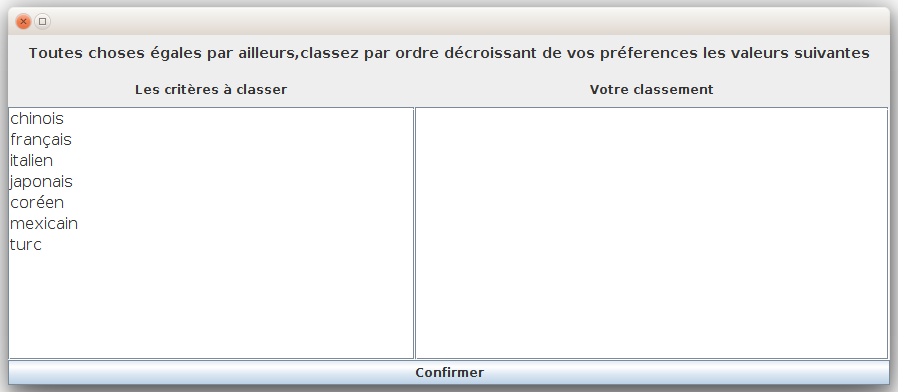
\includegraphics[width=4in]{Figures/pref.png}
%%				\caption{\label{fig:pref} Interface for entering an order of preference. Example for the cuisine criteria}
%%			\end{figure} 
%			
%			
%		\subsubsection{Operational hypotheses}
%		We therefore formulate the following operational hypotheses:
%		\begin{itemize}
%			\item \textit{\textbf{H1}}: The complementary and similar behaviors of virtual agents are perceived by participants.
%				
%				\subitem $\circ$ The behaviors of dominance attributed by participants to agents are \textit{significantly different} from those they have attributed to them selves.
%				\subitem $\circ$ The behaviors of dominance attributed by the participants to the agents are \textit{similar} to the those they have attributed to them selves.
%				
%				\item \textit{ \textbf{H2}}: Negotiators achieve a greater common gain when negotiators establish a complementary dominance relationship.
%					\subitem $\circ$ The restaurant chosen at the end of the negotiation has a satisfaction value which is significantly more important for the preferences of both negotiators in the complementary condition compared to the other conditions. 
%					
%					\item[$\bullet$] \textit{\textbf{H3}}: Negotiation converges more quickly when negotiators have a complementary dominance relationship.
%						\subitem $\circ$ Participants will engage in more rounds of negotiations to find a compromise in the similar and neutral condition compared to the complementary condition.
%						
%					\item \textit{\textbf{H4}}: The participant feels more comfortable with a partner who expresses complementary behaviors of dominance.
%						\subitem $\circ$ The perceived \emph{comfort} scores are higher for the complementary agent and control than for the similar agent.
%						\subitem $\circ$ Participants find it easier to negotiate with the complementary agent than with other agents.
%						
%					\item \textit{\textbf{H5}}: Complementarity in the dominance relationship increases appreciation between negotiators.
%						\subitem $\circ$ Participants will perceive the complementary agent as significantly more pleasant than the similar or neutral agent.
%								
%		\end{itemize}
%		
%		
%	\section{Results}
%	\label{sec:res}
%	We conducted an intra-subject study in which 63 participants took part. However, two participants were excluded because they did not meet the required conditions (incorrect answers to the majority of the manipulation check questions).
%	Therefore, our statistical study was conducted on the remaining 61 participants. 
%	
%		\subsection{Evaluation of the agent's behaviors}
%			To study the differences between the behaviors of dominance expressed by agents and participants, non-parametric statistics were used because the normality of the data could not be ensured. For the main analysis, the Wilcoxon signed rank test was applied to assess each of the four behaviors.
%			\begin{table*}[t]
%				\caption{Difference in perception of dominance between the agent and the participant for each behavior} 
%				\centering
%				
%				\begin{tabular}{p{1.5cm}  p{2.2cm}  p{1.5cm}  p{1.5cm}  p{1.5cm}  p{1.5cm}  p{1.5cm}}
%					\hline\hline
%					\textbf{Agent}& Evaluation & \textbf{D1} & \textbf{D2} & \textbf{D3} & \textbf{D4} \\ 
%					\hline
%					
%					\multirow{3}{*} {\textbf{Comp.}}  &  Z-Wilcoxon  & -4.61 & -5.3 & -6.28 & -0.43 \\ 	
%					& p-value & 2.88E-06 & 7.31E-08 & 1.42E-10 & \textbf{0.65 }\\ 
%					& Effect size & -0.29 & -0.34 & -0.4 & -0.03\\ 
%					\hline
%					
%					\multirow{3}{*} {\textbf{Similar}}  &  Z-Wilcoxon  & -1.57 & -2.21 & -1.45 & -1.33\\ 	
%					& p-value & 0.11 & \textbf{0.024} & 0.14 & 0.17 \\ 
%					& Effect size & -0.1 & -0.14& -0.09 & -0.08 \\ 
%					\hline
%					
%					\multirow{3}{*} {\textbf{Neutral}}  &  Z-Wilcoxon  & -6.23 & -5.72 & -7.056 & -0.77\\ 	
%					& p value & 2.52E-10 & 6.85E-09 & 8.19E-13 & \textbf{0.4351} \\ 
%					& Effect size & -0.4 & -0.36 & -0.45 & -0.049 \\ 
%					\hline \hline
%					
%				\end{tabular}
%				
%				\label{tab:domPercption}
%			\end{table*}
%			
%	\subsubsection{Perception of complementarity of dominance}
%	
%	At the end of each negotiation, we asked participants to report on their behaviors of dominance expressed during the negotiation. For each dimension, we compared participants' perceptions of their behaviors with those expressed by the complementary agent. The descriptive statistics are presented in figure \ref{fig:comp}.
%	
%	
%	The results of Wilcoxon's analysis revealed that participants perceived a significant difference between their behaviors and those of the agent as presented in the table \ref{tab:domPercption}. This difference concerns the behaviors \textbf{D1, D2} and \textbf{D3}. However, no significant differences were perceived for leadership behavior in negotiation \textbf{D4}.
%	
%		\begin{figure}[h]
%			\centering
%			% this is wide enough
%			\subfloat [Perception score of dominance behaviors]{
%				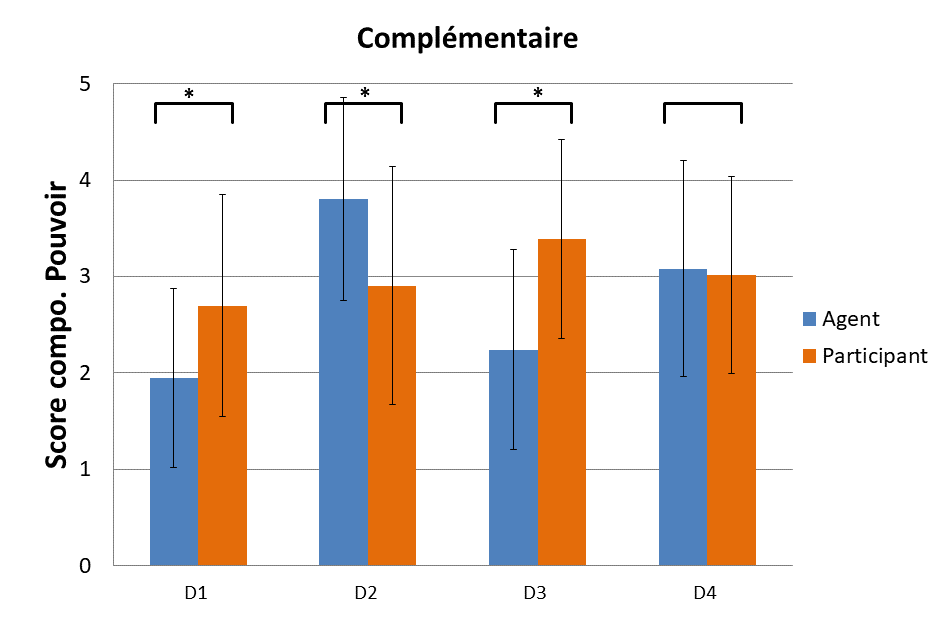
\includegraphics[clip=false,width=0.9\columnwidth]{figs/comPow.PNG}
%			}
%			
%			% this has a too narrow subfigure
%			\subfloat[Mean and standard deviation for the behavior of dominance perceived]{
%				\begin{tabular}{l c c c c c c}
%					\hline\hline
%					\textbf{Agent} & Evaluation&  \textbf{D1} & \textbf{D2} & \textbf{D3} & \textbf{D4} \\
%					\hline
%					
%					\multirow{2}{*}{\textbf{Comp.} }& Mean & 1,94& 3,80 & 2,24 & 3,08 \\
%					& SD & 0,93 & 1,05 & 1,03 & 1,11 \\
%					
%					\hline
%					\multirow{2}{*}{\textbf{Part.}}& Mean & 2,69 & 2,94 & 3,4 & 3,02 \\
%					& SD & 1,14 & 1,23 & 1,03 & 1,02\\
%					\hline
%					\hline
%				\end{tabular}
%			}
%			\caption{Perception of behaviors of dominance  with the complementary agent Bob}
%			\label{fig:comp}
%		\end{figure}
%		
%		\subsubsection{Perception of similarity of dominance}
%		
%		We also analyzed the negotiators' behaviors during their interactions with Agent Arthur. Descriptive statistics have already shown a strong similarity in the perception of all behaviors (see figure \ref{fig:sim}). We completed the study with a comparison of Wilcoxon which confirmed the absence of significant difference between the agent Arthur and  participants behaviors of dominance as presented in the table \ref{tab:domPercption}.  
%		
%			\begin{figure}[!tb]
%				\centering
%				% this is wide enough
%				\subfloat[Score of dominance behaviors]{
%					\centering
%					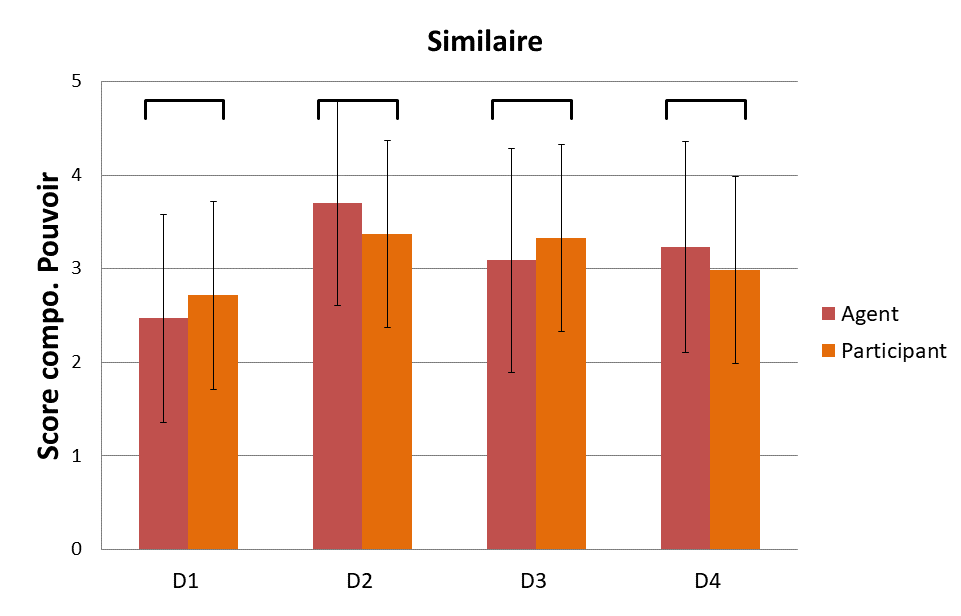
\includegraphics[clip=false]{figs/simPow.PNG}
%				}
%				
%				%\vspace{1em}
%				% this has a too narrow subfigure
%				\subfloat[Mean and standard deviation for the behavior of dominance perceived]{
%					\centering
%					\begin{tabular}{l c c c c c c}
%						\hline\hline
%						\textbf{Agent} & Evaluation& \textbf{D1} & \textbf{D2} & \textbf{D3} & \textbf{D4} \\
%						\hline
%						
%						\multirow{2}{*}{\textbf{Simil.}}& Mean & 2,47 & 3,70 & 3,09 & 3,23 \\
%						& SD & 1,11 & 1,10 & 1,19 & 1,12 \\
%						
%						\hline
%						\multirow{2}{*}{\textbf{Part.}}& Mean & 2,71 & 3,37 & 3,33 & 2,98 \\
%						& SD & 1,06 & 1,03 & 1,06 & 1,09\\
%						\hline \hline
%						
%					\end{tabular}
%				}
%				\caption{Perception of behaviors of dominance with the similar agent Arthur}
%				\label{fig:sim}
%			\end{figure}
%			
%		\subsubsection{Behaviors of the neutral agent}
%		
%		We conducted the same statistical studies to analyze the perception of the neutral agent's behaviors. The descriptive analysis presented in Figure \ref{fig:neutral} shows that participants perceived that the agent was adopting a complementary strategy for the behaviors \textbf{D1}, \textbf{D2} and \textbf{D3}. However, no significant differences were perceived for the \textbf{D4} behavior.
%		
%			\begin{figure}[!tb]
%				\centering
%				% this is wide enough
%				\subfloat[Score of dominance behaviors]{
%					
%					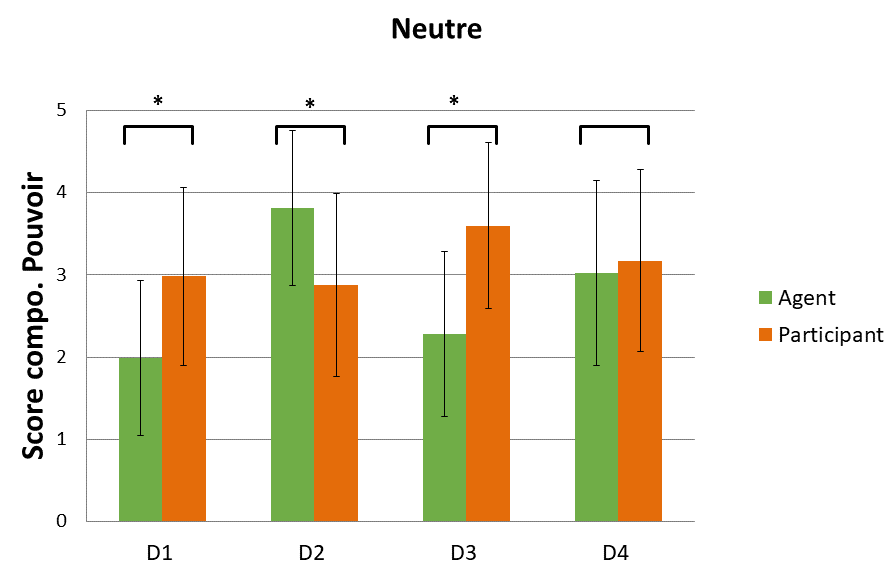
\includegraphics[clip=false]{figs/neutrePow.PNG}
%				}
%				
%				%\vspace{1em}
%				% this has a too narrow subfigure
%				\subfloat[Mean and standard deviation for the behavior of dominance perceived]{
%					
%					\begin{tabular}{l c c c c c c}
%						\hline\hline
%						\textbf{Agent} & Evaluation& \textbf{D1} & \textbf{D2} & \textbf{D3} & \textbf{D4} \\
%						\hline
%						
%						\multirow{2}{*}{\textbf{Neutre}}& Moyenne & 1,99 & 3,81 & 2,28 & 3,02 \\
%						& Ecart-type & 0,94 & 0,94 & 1,01 & 1,12 \\
%						
%						\hline
%						\multirow{2}{*}{\textbf{Part}}& Moyenne & 2,98 & 2,88 & 3,60 & 3,17 \\
%						
%						& Ecart-type & 1,08 & 1,12 & 1,01 & 1,10 \\
%						\hline \hline
%						
%					\end{tabular}
%					
%				}
%				\caption{Behaviors of the neutral agent Kevin}
%				\label{fig:neutre}
%			\end{figure}
%		
%	\subsection{Common gain}
%		We analysed the impact of the dominance on the joint gain during the various negotiations. First, we asked the participants their degree of satisfaction regarding the chosen the chosen restaurant. We completed this analysis with an objective study in which we calculated the satisfaction score of the chosen restaurant based on the preferences of the participant and the agent. All the results are presented in Appendix \ref{chap:Appendix}.
%		
%			\begin{figure}[h]
%			
%			\centering
%			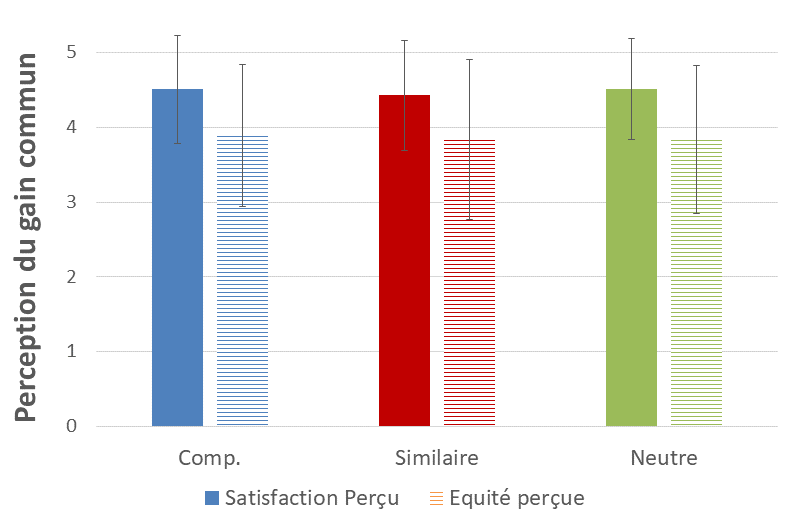
\includegraphics[width= 0.65 \linewidth,clip=false]{figs/percpGain.PNG}
%			\caption{Perception of the joint gain for all the agents \textit{No significant difference was observed}}
%			\label{fig:gainCom}
%		\end{figure}
%	
%	\subsubsection{Perception of common gain}
%	Participants were asked to rate their satisfaction with the restaurant they chose with the agent.
%	
%	The results are presented in figure \ref{fig:gainCom}. First, descriptive statistics show that, on average, participants were satisfied with the restaurant chosen for all negotiations. The scores are above average for all agents (values range from \emph{3.83} to \emph{4.5} on a scale of \emph{5}). 
%	
%	In addition, we analyzed whether participants were significantly more satisfied with the restaurant chosen during the negotiation with Agent Bob than with the other agents. We performed a test of Wilcoxon's signed ranks because the normality of the data could not be assured. The analysis showed no significant difference in the perception of gain and fairness in the choice of restaurant between the different agents. 
%	
%	\subsubsection{Analysis of the common gain achieved} 
%	Regarding the objective analysis of the common gain achieved at the end of each negotiation, we used the preferences of the participants and the agents with whom they had interacted as presented in the section \ref{sec:proto}. 
%	Based on each negotiator preferences, we calculated their satisfaction of the restaurant chosen. We then calculated the common gain achieved at each negotiation as \textbf{the average of the satisfaction values} of the two negotiators. The results obtained for each agent are presented in Figure \ref{fig:gain}. 
%	
%				\begin{figure}[h]
%			
%			\subfloat[Score of the common gain achieved for all agents \textit{Populations grouped with $(*)$ are significantly different}]{
%				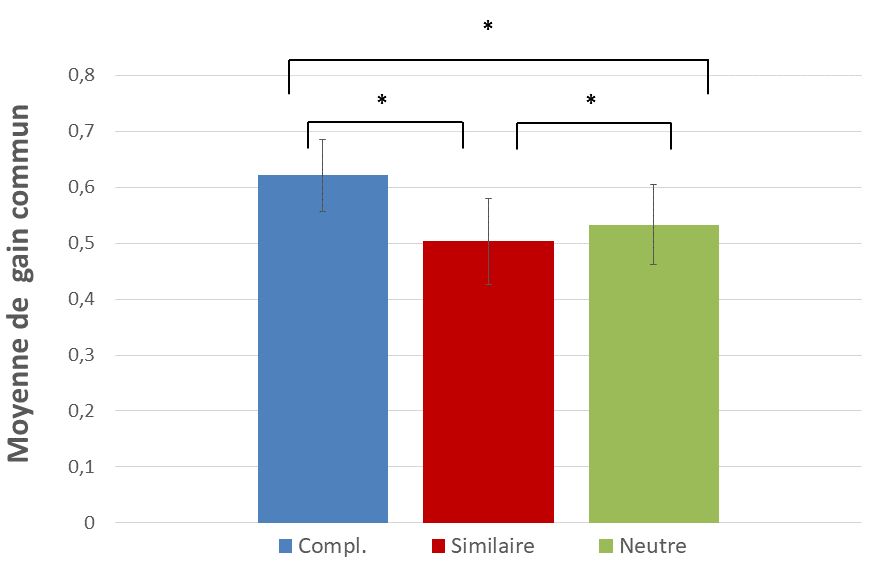
\includegraphics[clip=false]{figs/gainCommun.PNG}}
%			
%			\subfloat []{
%				\centering
%				\begin{tabular}{l c c c}
%					\hline
%					\hline
%					\textbf{ }& \textbf{Comp.} & \textbf{Similar} & \textbf{Neutral} \\ 
%					\hline
%					\newline Mean & 0.62& 0.5 & 0.53 \\
%					\newline SD & 0.06 & 0.08 & 0.07 \\
%					\hline
%					\hline
%				\end{tabular}
%			}
%			\caption{Common gain achieved during the negotiation}
%			\label{fig:gain}
%		\end{figure}
%		
%	Satisfaction values are above average for all agents. It should be recalled that the satisfaction values are normalized within a range of $[0, 1] $. We examined whether negotiators had achieved a greater joint gain by negotiating with the complementary agent, compared to other agents. Because the  distribution of data is normal, we applied a T-test to compare each pair of agents. The results obtained are presented in figure \ref{fig:gain}. The analysis of variance showed a significant interaction between the dominance relationship and the common gain achieved during the negotiations. Indeed, participants achieved a significantly higher common gain by negotiating with the complementary agent than with the similar agent (\emph{t= 8.9, p < 0.01}). The same difference was perceived when compared with the neutral agent (\emph{t= 6.4, p < 0.01}).
%	
%	In addition, participants achieved a better common gain with the neutral agent than with the similar agent (\emph{t= 2.3, p = 0.02}).
%	
%	\subsection{Number of negotiation turns}
%	
%	For each negotiation, we collected the number of utterances stated. Our purpose is to analyze the impact of the dominance on the number of utterances stated before reaching a compromise. 
%	
%	The descriptive statistics are presented in Figure \ref{fig:tour}. A parametric test was used because the data have a normal distribution. The results show that the negotiation converged significantly faster when participants negotiated with the complementary agent compared to the similar agent (\emph{t= 2.7, p = 0.003}). Similarly, negotiation converges more quickly with the neutral agent than with the similar agent (\emph{t= 4.43, p < 0.01}).  The results are presented in Appendix \ref{chap:Appendix}.
%	
%	However, no significant difference was perceived between the complementary agent and the neutral agent (\emph{t=1.3, p = 0.09}).
%
%		
%		\begin{figure}[!tbh]
%			
%			\subfloat[Number of negotiation rounds during a negotiation for all agents \textit{the populations grouped with $(*)$ are significantly different}] {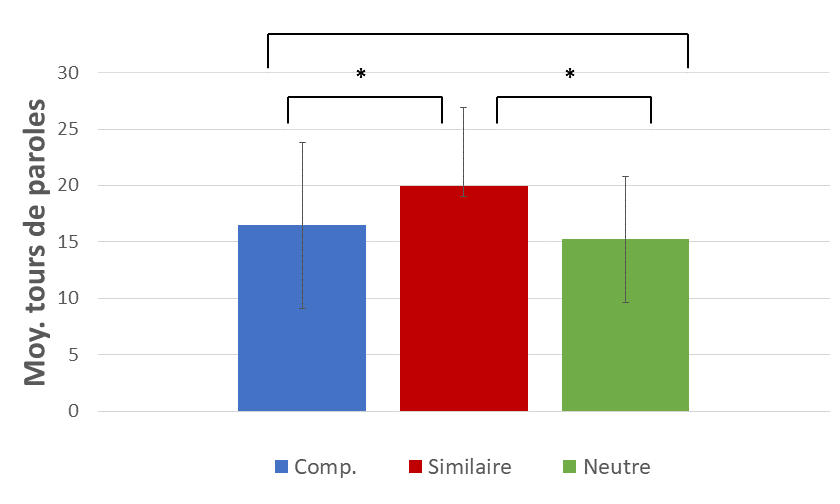
\includegraphics{figs/tours.PNG}}
%			
%			
%			\subfloat[Number of utterances stated for each negotiation]{
%				\centering
%				\begin{tabular}{ l c c c }
%					\hline
%					\hline
%					\textbf{ }& \textbf{Comp.} & \textbf{Similar} & \textbf{Neutral} \\ 
%					\hline
%					\newline Mean & 16.61& 19.94 & 15.13 \\
%					\newline SD & 7.38 & 6.87 & 5.6 \\
%					\hline
%					\hline
%				\end{tabular}
%			}
%			\caption{Results obtained for H3.}
%			\label{fig:tour}
%		\end{figure}
%%	
%	
%	\subsection{Comfort during negotiation}
%	
%	The descriptive statistics are presented in the table \ref{tab:comfort}. Globally, participants felt comfortable with all agents.
%	The scores of compfort enunciated by participants are 3.4 higher (on a 5-point scale) for all agents. On the contrary, the anxiety scores are 2 lower (on a 5-point scale) for all agents. 
%	
%	In order to analyse the possible differences in perceived comfort, we used a non-parametric test because normality could not be ensured. The Wilcoxon signed rank test was applied to analyze whether participants felt more comfortable with the complementary agent than with other agents. (See results in appendix \ref{chap:appendix}). 
%	The results show that participants felt more comfortable with the complementary agent compared to the similar agent (\emph{Z= -2.73, p = 0.002})
%	with a small size effect (\emph{e = -0.1}). However, no significant difference was perceived between the complementary agent and the neutral agent. 
%	
%	\begin{figure}[h]
%	
%	\subfloat[Comfort score that participants felt for all agents. \textit{the populations grouped with $(*)$ are significantly different}]{
%		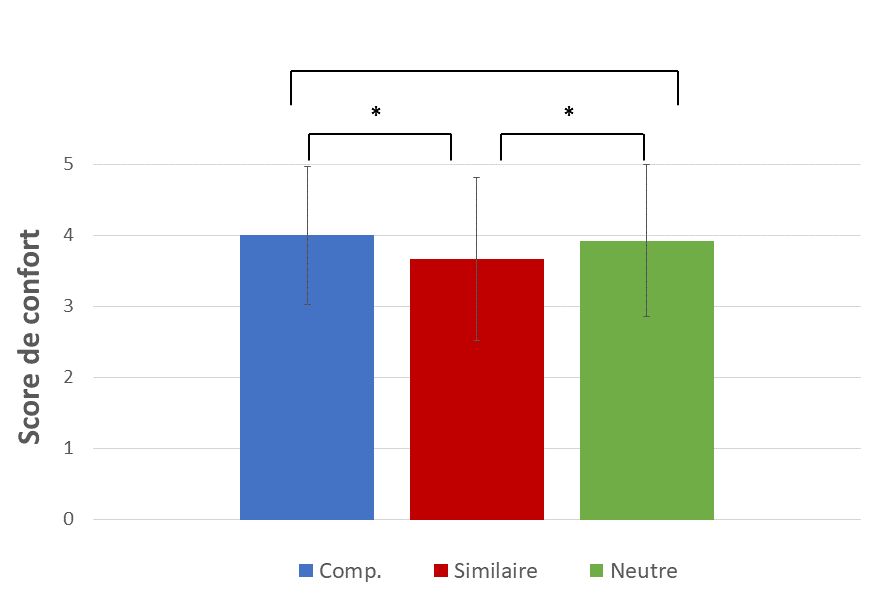
\includegraphics[clip=false]{figs/confort.PNG}
%	}
%	
%	\subfloat[The effect of the dominance on the comfort felt during negotiation]{
%		\centering
%		\begin{tabular}{ l l c c c  }
%			\hline\hline
%			\textbf{ }& & \textbf{Comp.} & \textbf{Similar} & \textbf{ Neutral} \\ 
%			\hline
%			\newline \newline\multirow{2}{*} {Relaxed} & Mean &3.79 & 3.47 & 3.79 \\
%			\newline  & SD & 1 & 1.2 & 1 \\
%			\hline
%			
%			\newline \newline\multirow{2}{*} {Anxious} & Mean & 1.79 & 2.13 & 1.93 \\
%			\newline  & SD & 7.38 & 6.87 & 5.6 \\
%			\hline\hline
%		\end{tabular}
%	}
%	\caption{Result of the analysis of comfort during negotiation}
%	\label{tab:confort}
%\end{figure}
%
%	\subsection{Appreciation}
%		Descriptive statistics on the appreciation scores are presented in Figure \ref{fig:app}. Overall, scores are centered around 3.7 (on a scale of 5). The analysis of variance shows the effect of the dominance relation on the perception of appreciation. The results are presented in appendix \ref{chap:appendix}.
%		
%				\begin{figure}[h]
%				
%				\subfloat[Appreciation score that participants felt for all agents. \textit{the populations grouped with $(*)$ are significantly different}]{
%					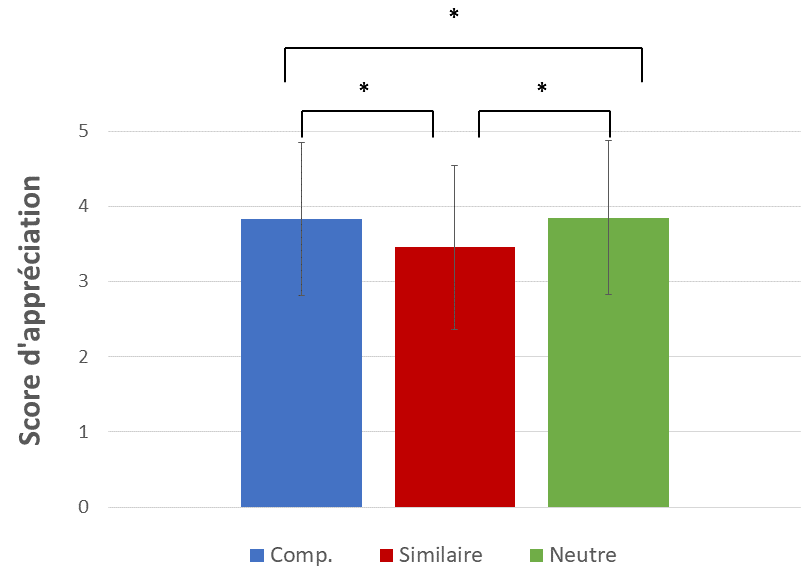
\includegraphics[clip=false]{figs/appreciation.PNG}
%				}
%				
%				\subfloat[The effect of the dominance relation on perceived appreciation]{			
%					
%					\begin{tabular}{ l c c c c c }
%						\hline\hline
%						\textbf{Agent}& \textbf{Comp.} & &  \textbf{Similar} & & \textbf{Neutral} \\ 
%						\hline
%						\newline Moy. & 3.83 & &3.46 & & 3.85 \\
%						\newline SD & 1.01 & & 1.09& &  1.02 \\
%						\hline\hline
%						
%					\end{tabular}
%				}
%				\caption{Perception of appreciation}
%				\label{fig:app}
%			\end{figure}
%			
%		The Wilcoxon signed rank test shows that the complementary agent was perceived as significantly more pleasant than the similar agent (\emph{p < 0.01, Z=-3.17}). In addition, the neutral agent was also perceived as more pleasant than the similar agent (\emph{p < 0.01, Z = -3.3}). However, no difference was perceived between the complementary agent and the neutral agent (\emph{p = 0.6, Z = -0.31}).
%		
%		We also looked at the ease of collaboration between the participant and the agent. Indeed, we asked participants to report on the degree of ease of negotiation with the agent. The results are presented in figure \ref{fig:ease}. In general, participants found that negotiating with the complementary agent was easy (\emph{M=4, SD = 1}) as well as with the neutral agent (\emph{M=3.9, SD =0.99}). Participants perceived negotiation with the similar agent as less easy (\emph{M=3.16, SD = 1.06}). 
%		
%		Then, we analysed whether this difference in their perceptions was significant. As the data are not normally distributed, we applied the Wilcoxon signed rank test. The results show that participants found that negotiating with the similar agent was significantly less comfortable compared to the complementary agent (\emph{p < 0.01, Z = -3.86} with a medium size effect \emph{e = -0.35}) and the neutral agent (\emph{p < 0.01, Z = -3.61} with a medium size effect \emph{e = -0.32}).
%		However, no difference was perceived between the complementary agent and the neutral agent.
%		
%			\begin{figure}[h]
%			
%			\subfloat[Evaluation of collaboration during negotiation. \textit{the populations grouped with $(*)$ are significantly different}]{
%				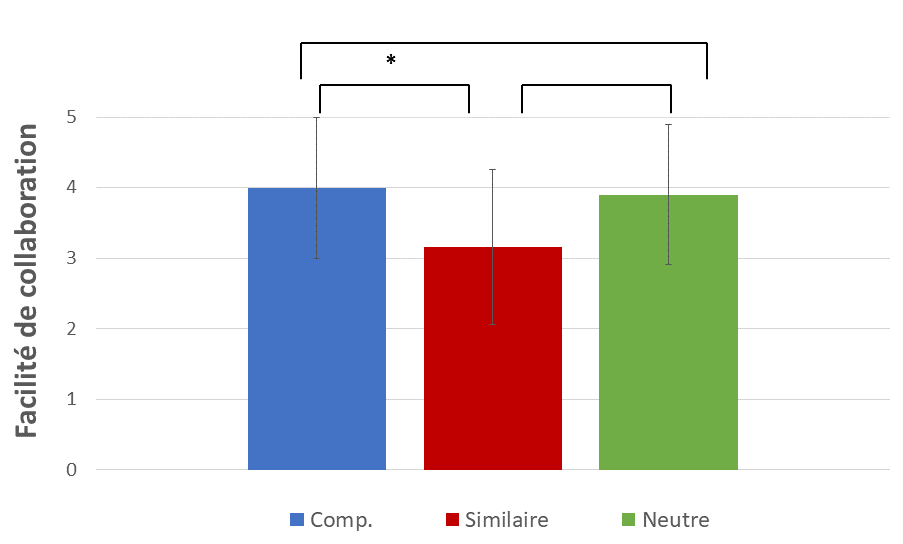
\includegraphics[clip=false]{figs/aisee.PNG}
%			}
%			
%			\subfloat[Impact of dominance on the ease of negotiation]{
%				\centering
%				\begin{tabular}{ l c c c c c }
%					\hline\hline
%					\textbf{ }& \textbf{Comp.} & &  \textbf{Similar} & & \textbf{Neutral} \\ 
%					\hline
%					\newline Mean & 4 & & 3.16 & & 3.9 \\
%					\newline SD & 1 & & 1.09  & & 0.99   \\
%					\hline\hline
%					
%				\end{tabular}
%			}
%			\caption{Results for ease of collaboration during negotiation.}
%			\label{fig:aise}
%		\end{figure}
%	
%	
%	\section{Complementary analysis}
%	In section \ref{sec:Dom}, we presented the dominance as an interpersonal relationship that develops during the interaction. 
%	Therefore, in addition to the personality trait, an individual is influenced by the environment of the interaction (e. g. context of the interaction, social role...). These different parameters will create a certain dominance relationship that may vary from one interaction to another.  
%	In order to check whether participants produced different dominance behaviors during the different negotiations, we collected the agent's perception of the interlocutor's dominance behaviors.  The results are presented in figure \ref{fig:dom}.
%	
%	For the same participant, we analyzed the variance of dominance behaviors across the three negotiations. To do this, we used the Wilcoxon signed rank test because the normality of the data could not be ensured. 
%	
%	The results show that participants' dominance behaviors varied from one interaction to another. Indeed, the Wilcoxon test reveals a significant difference between the behavior perceived by the complementary agent and the similar agent (\emph{p<0.01, Z = -3.35}). These same results are observed by comparing the perception of the complementary agent and the neutral agent (\emph{p< 0.01, Z = -3.88}).
%	However, no difference between the similar agent and the neutral agent was observed (\emph{p = 0.6, Z = 0.44}). 
%	
%	These results suggest that participants have adopted a different negotiation strategy based on the relationship established with the agent.
%%		
%%		\begin{figure}[h]
%%		
%%		\subfloat[Evaluation of participants' perceived dominance behaviours by agents. \textit{the populations grouped with $(*)$ are significantly different }]{
%%			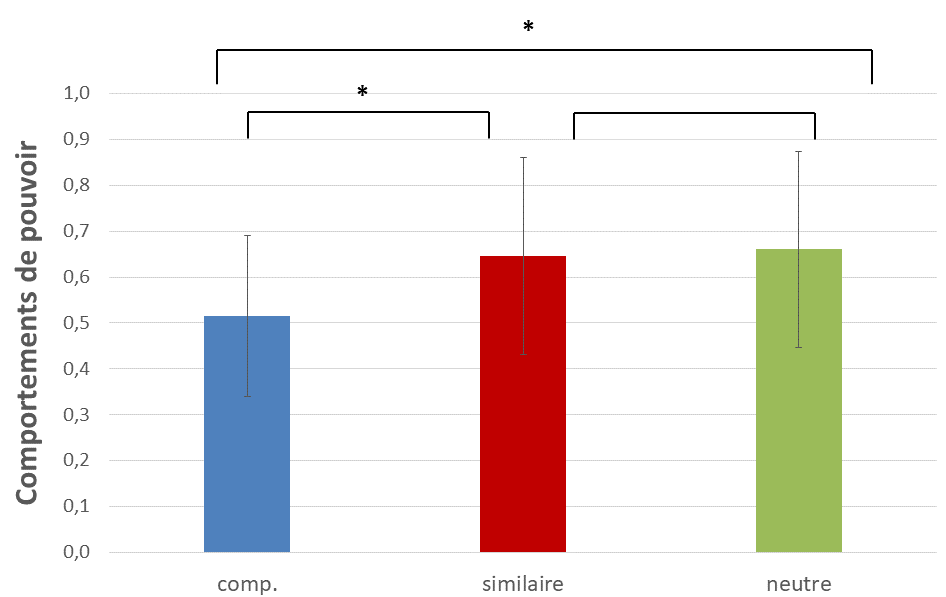
\includegraphics[clip=false]{figs/pow.png}
%%		}
%%		
%%		\subfloat[Agent's perception of the dominance behaviours expressed by participants]{
%%			\begin{tabular}{ l c c c c c }
%%				\hline
%%				\hline
%%				\textbf{ }& \textbf{Comp.} & &  \textbf{Similar} & & \textbf{Neutral} \\ 
%%				\hline
%%				\newline Moy. & 0.51 && 0.64 && 0.66 \\
%%				\newline SD & 0.17 && 0.21 && 0.219   \\
%%				\hline
%%				\hline
%%			\end{tabular}
%%		}
%%		\caption{Results for the variation of dominance behaviours through interactions.}
%%		\label{fig:dom}
%%	\end{figure}
%
%\section{Discussion}
%\label{sec:discussion}
%In general, all our assumptions have been validated. These results support the validity of our collaborative negotiation and theory of mind model in agent/human interaction.   
%
%\subsection{Perception of agent behaviors}
%Our H1 hypothesis (\textit{the complementarity and similarity behaviours of virtual agents are perceived by participants}) is partially validated. 
%
%Four dominant behaviours were taken into account to measure the negotiation strategy. 
%Participants were able to distinguish a significant difference from three out of four behaviours between their strategies and that of the complementary agent.
%
%Indeed, participants perceived a difference between their levels of level and concessions \textbf{D3}, \textbf{D2}, as well as the consideration of the other's preferences \textbf{D1}. However, no difference was perceived regarding leadership behaviors during the negotiation \textbf{D4}. 
%
%We then analyzed the behavior of the neutral agent. The agent was perceived as adopting dominance behaviors significantly complementary to those of users for the behaviours \textbf{D1}, \textbf{D2} and \textbf{D3}. 
%However, no difference was perceived in the behaviors related to \textbf{D4} between the neutral agent and the participants. 
%
%We studied the data to understand why participants did not perceive any difference in leadership behaviors. 
%
%Concerning the complementary agent, the leadership behaviors could be masked because of his adaptation strategy which modifies his dominance behaviours at each speaking turn.
%
%In addition, the collaborative aspect of bargaining may have reduced the perception of leadership in bargaining, which may explain the case of the neutral agent. 
%
%Finally, the lack of results for the two agents leads us to question the items proposed to measure leadership. 
%It would be interesting to do a post-hoc evaluation to ask participants what kind of behaviors they would relate to leadership during the negotiation.
%
%At the same time, participants perceived a similarity between their behaviors and those of the similar agent. On average, for each behavior, the values assigned in self-attribution and hetero evaluation are very close. In addition, the absence of significant differences supports this result. We are aware that the absence of difference is not an insurance of similarity of perception. However, it is difficult to find a statistical calculation that ensures similarity between two populations.
%
%More generally, the results obtained support the consistency of our decision-making model both on the perception of dominant behaviors and on the agent's ability to perceive and adapt correctly to the other person's behaviors.  
%
%Moreover, the perception of the neutral agent's behaviors as complementary to those of the participants argues that the interpersonal relationship of dominance that develops during the interaction is complementary \cite{burgoonnonverbal}. Indeed, independently of the other two agents where we had manipulated the agent's adaptation, in the neutral condition the agent does not adapt to the participant's behaviors. Nevertheless, the results show that the participant has adapted to the behaviors exhibited by the agent and has thus established an interpersonal relationship of complementary dominance.
%
%\subsection{Common gain}
%Our second hypothesis (\textit{negotiators achieve a greater common gain when they establish a complementary dominance relationship.}) is validated. 
%
%First, we asked participants to share their preferences on the restaurant chosen for each negotiation.
%In general, participants were satisfied with the final choice and found it fair for all negotiations. 
%By analyzing the satisfaction value of the chosen restaurant for the participants' preferences (see table \ref{tab:gainPerceptive}), the values were around 0.7 (\emph{min =0.69, max = 0.73}). 
%
%However, by analyzing the satisfaction value for the agent's preferences, on average, only the complementary agent was able to converge on a restaurant that respects his preferences (\emph{M = 0.53, SD = 0.2}). 
%
%%	\begin{table}
%%	\centering
%%	\caption{Average of the satisfaction values of the restaurant chosen for each negotiator} 
%%	\begin{tabular} {lcccccccc}
%%		\hline
%%		\hline
%%		& \multicolumn{2}{c}{Comp.} & & \multicolumn{2}{c}{Similar}& & \multicolumn{2}{c}{Neutral} \\ % column 4 blank, for spacing
%%		\cline{2-3} \cline{5-6} \cline{8-9} % horizontal lines connecting cols. 2-3, 5-6
%%		& Part. & Agent & & Part. & Agent & &  Part. &Agent \\ \hline
%%		Mean &0,71 & 0,53 & &  0,69 & 0,33 & & 0,73 & 0,34 \\
%%		SD & 0,2 & 0,24 & &  0,18 & 0,19 & & 0,18 & 0,16 \\
%%		\hline
%%		\hline
%%	\end{tabular}
%%	\label{tab:gainPerceptif}
%%	
%%\end{table}
%
%This is due to the fact that negotiators did not communicate well during the negotiation. As a result, the negotiation was taking longer, causing the $Self$ concession function to fall. As a result, the agent made more concessions and ended up accepting a restaurant with a low level of satisfaction (\emph{M = 0.33, SD = 0.18}).
%
%Concerning the neutral agent, which is not very dominant, it is normal that in most cases, the concession curve eventually decreased leading the agent to make significant concessions. This explains the average satisfaction achieved by the neutral agent (\emph{M = 0.34, SD = 0.16}).
%
%This analysis confirms the results of the objective study conducted.
%For all negotiations, we compared the common gain and observed that it was significantly more important during negotiations with the complementary agent than with other agents. In addition, negotiators had better gains during negotiations with the neutral agent compared to the similar agent. This proves that the complementary relationship that developed during the negotiation with the neutral agent allowed for a better exchange of information. 
%
%These results confirm that negotiators communicate better and therefore negotiate better in a complementary dominance relationship.  
%
%
%\subsection{Turn of utterances}
%Our H3 hypothesis (\textit{Negotiation converges more quickly when negotiators have a complementary dominance relationship}) is validated. Indeed, negotiation converged on average more quickly when a complementary dominance relationship was established between the agent and the participant. Moreover, under the same condition, the common gain achieved by the negotiators was greater. Thus, these results support social psychology theories that interpersonal dominance relationships improve coordination and information exchange.
%
%
%As for the neutral agent, negotiation converged quickly for two reasons. First, with a dominance value initialized at 0.5, the agent had an average level of demand which facilitated the process of finding a compromise. 
%Second, according to our results, in this condition, a complementary dominance relationship had been established between the negotiators, which facilitated coordination. 
%
%In conclusion, the interpersonal dominance relationship improves coordination and information exchange that results in short and more effective negotiation processes.
%
%\subsection{Appreciation of the agent}
%Our hypotheses H4 (\textit{The negotiator feels more comfortable with a partner who expresses complementary behavior}) and H5 (\textit{Complementarity in the dominance relationship increases the appreciation between negotiators.}) are validated. 
%
%For appreciation, the scores are above average for all agents. This may reflect a slight positive bias towards agents. However, the analysis of the differences revealed that participants significantly appreciated the negotiation with the complementary agent more than the similar agent. Similarly, participants felt that the neutral agent was also more pleasant than the similar agent. 
%
%In addition, we analyzed the comfort felt during the negotiation. Overall, participants felt relaxed during the negotiation and found the negotiation comfortable with all agents.  
%
%The analysis of variance revealed that participants felt more comfortable with the complementary agent than with the similar agent. However, no difference was perceived between the complementary agent and the neutral agent, and between the neutral agent and the similar agent.
%
%In addition to comfort, we analyzed the ease of collaborating with the agent during the negotiation. The results show that participants perceived the negotiation process to be easier with the complementary agent and the neutral agent than with the agent adopting a similar strategy to their own. 
%
%These results confirm our assumptions. Participants prefer to negotiate with a partner with whom they have established a complementary relationship rather than with a negotiator who exhibits similar dominant behaviors. 
%
%
%
%%----------------------------------------------------------------------------------------
%					
%\section{Conclusion}
%
%For this fourth study, our objective was to study the effect of the dominance relationship on bargaining between an agent and a human participant. We have based ourselves on the work of Tienders and Wiltermuth \cite{wiltermuth2009benefits,tiedens2003power} which asserts that complementarity in the dominance relationship had a positive impact on negotiation. 
%
%We implemented three bargaining agents adopting three different strategies, a complementary agent, a similar agent and a neutral agent. 
%63 participants took part in collaborative negotiations with these agents to find a restaurant that meets their preferences. 
%
%The results confirmed most of our assumptions and allowed us to go further in the analysis of dominance behaviors in negotiation. 
%
%First, we were able to validate our theory of mind model through interaction with a human user. 
%The results show that participants were able to perceive a difference in the strategies adopted by the agents. This allows us to validate the robustness of our model's predictions. 
%
%In addition, all hypotheses relating to the positive effect of the complementary dominance relationship have been validated. When negotiators established a complementary dominance relationship, they achieved a better common gain and those in a shorter time frame compared to other configurations. The negotiation was perceived as more pleasant and comfortable and the negotiators seemed to collaborate better. 
%
%The results also revealed behaviors that support social psychology work. Indeed, by analyzing the behaviors expressed during negotiations with the neutral agent, we realized that a complementary relationship of dominance had developed between the negotiators. These results support Dunbar and Burgoon's definition of \cite{dunbar2005perceptions}, which asserts that the dominance relationship is necessarily complementary. In addition, since the dominance relationship is interpersonal, it is established during the interaction. This point was also validated by our analyses, which allowed us to show that participants adopted different dominance behaviors from one negotiation to another. This suggests that negotiators should adapt to their interlocutor to define a dominance relationship specific to the interaction. 			
%----------------------------------------------------------------------------------------
%	BIBLIOGRAPHY
%----------------------------------------------------------------------------------------

\printbibliography[title={Bibliography}] % Print the bibliography, section title in curly brackets

%----------------------------------------------------------------------------------------



\end{document}
